\hypertarget{dl_8c}{}\section{dl.\+c File Reference}
\label{dl_8c}\index{dl.\+c@{dl.\+c}}


Loading modules under linux.  


{\ttfamily \#include $<$kdbconfig.\+h$>$}\newline
{\ttfamily \#include $<$dlfcn.\+h$>$}\newline
{\ttfamily \#include $<$kdberrors.\+h$>$}\newline
{\ttfamily \#include $<$kdbmodule.\+h$>$}\newline
{\ttfamily \#include $<$stdlib.\+h$>$}\newline
{\ttfamily \#include $<$string.\+h$>$}\newline
Include dependency graph for dl.\+c\+:
\nopagebreak
\begin{figure}[H]
\begin{center}
\leavevmode
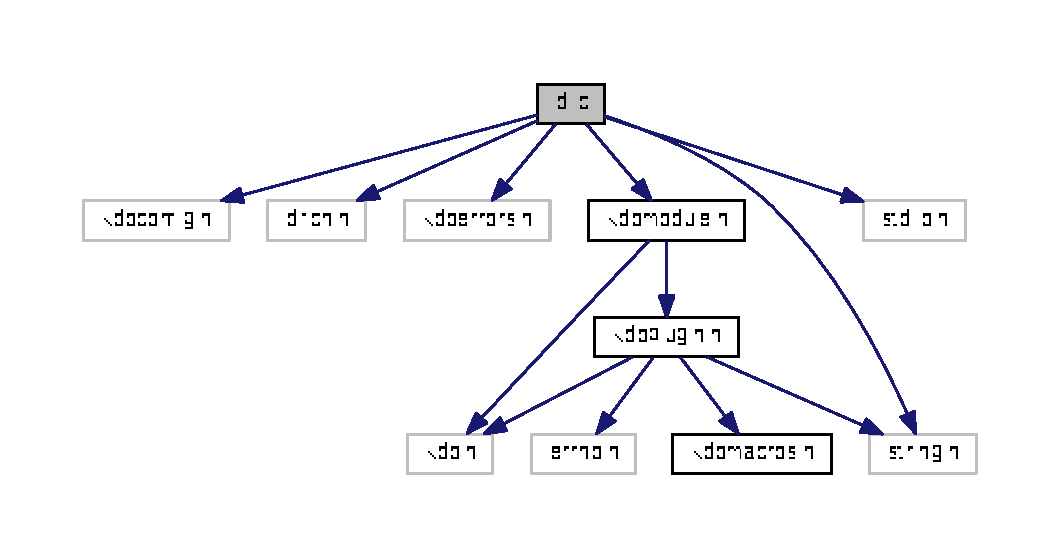
\includegraphics[width=350pt]{dl_8c__incl}
\end{center}
\end{figure}


\subsection{Detailed Description}
Loading modules under linux. 

\begin{DoxyCopyright}{Copyright}
B\+SD License (see L\+I\+C\+E\+N\+S\+E.\+md or \href{https://www.libelektra.org}{\tt https\+://www.\+libelektra.\+org})
\end{DoxyCopyright}
The name of the module will be libname. A .so will be appended. This file will be loaded.

The path were the plugins are located, e.\+g. /usr/src/elektra need to be added with L\+D\+\_\+\+L\+I\+B\+R\+A\+R\+Y\+\_\+\+P\+A\+TH.

The reason is that only L\+D\+\_\+\+L\+I\+B\+R\+A\+R\+Y\+\_\+\+P\+A\+TH also loads libraries which are seen by symlink only. That feature is needed for libelektra-\/default.

The buildsystem makes sure that dlfcn.\+h exists. 